\chapter{Design}

\section{User Interface}
The first section, \textit{User Interface}, presents the four user interface iterations. Each iteration is presented and the changes to the previous generation are highlighted.


\begin{figure}[H]
    \centering
    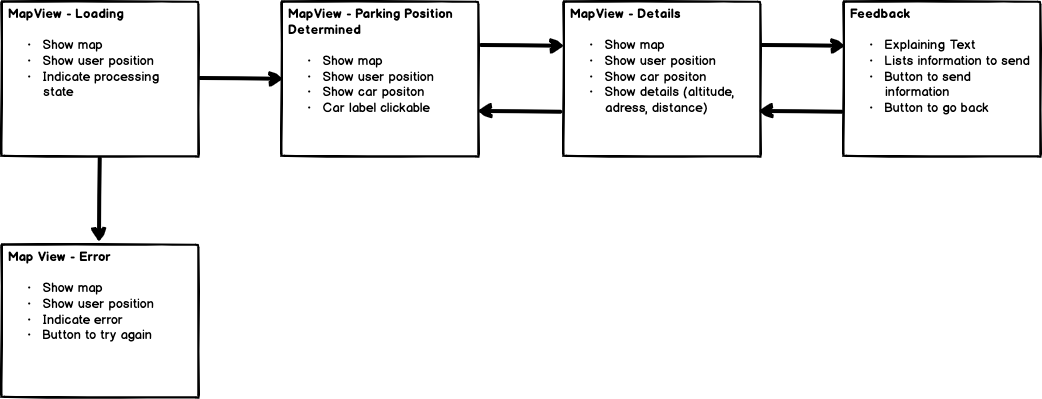
\includegraphics[width=\textwidth]{images/UI/Iteration1-Overview.png}
    \caption{Iteration 1 - Storyboard}
    \label{fig:i1story}
\end{figure}

\begin{figure}[H]
    \centering
    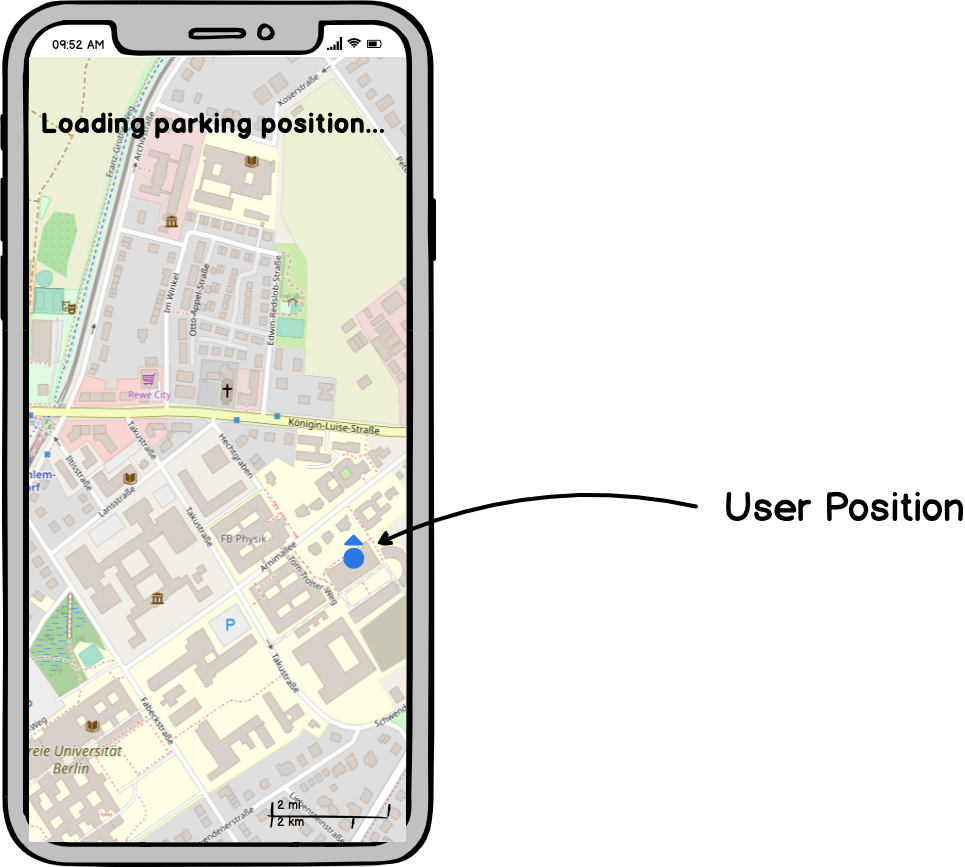
\includegraphics[width=0.5\textwidth]{images/UI/[I1V1]MapView-Loading.png}
    \caption{[I1V1] MapView - Loading}
    \label{fig:i1v1}
\end{figure}

\begin{figure}[H]
    \centering
    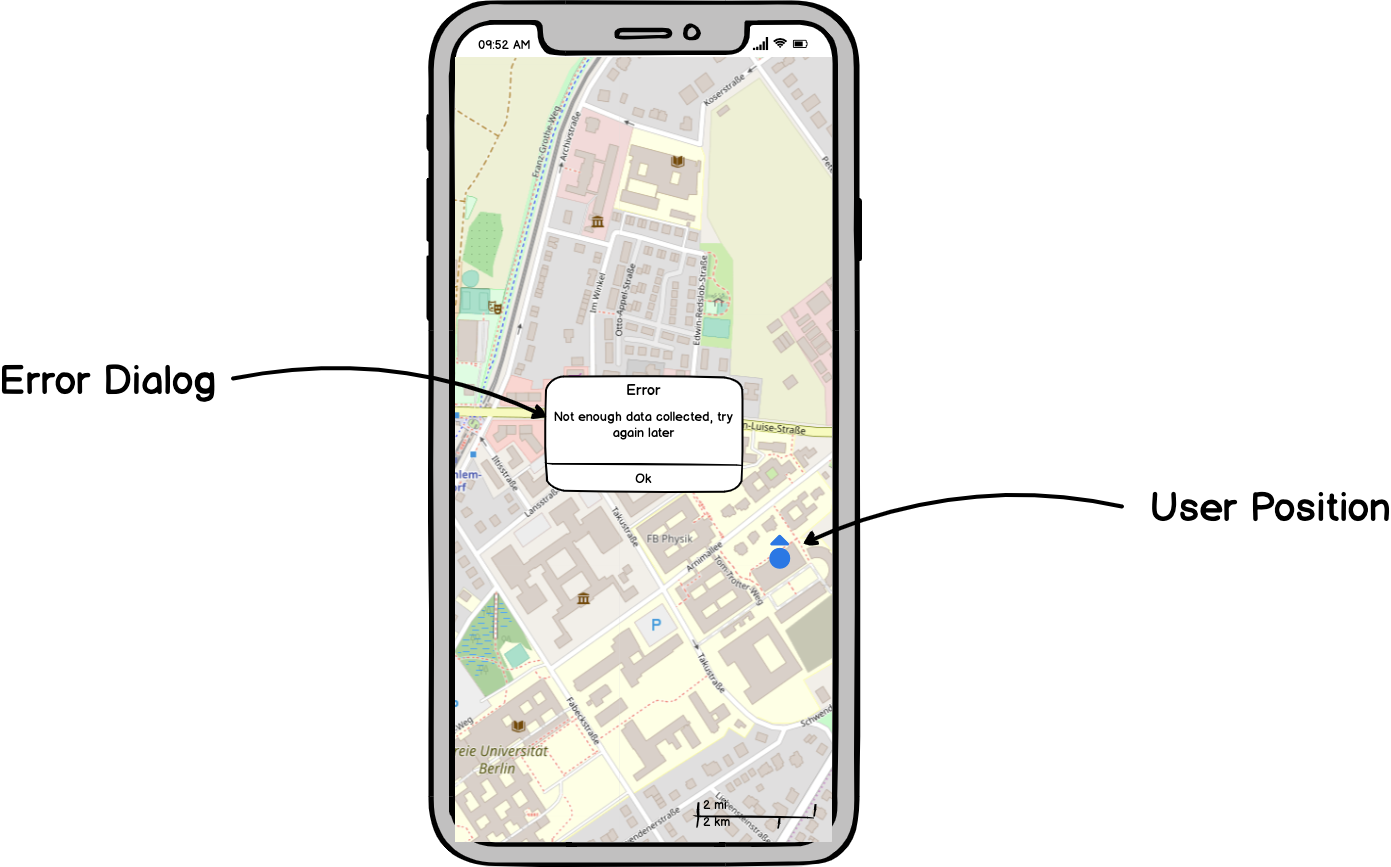
\includegraphics[width=0.75\textwidth]{images/UI/[I1V2]MapView-Error.png}
    \caption{[I1V1] MapView - Error}
    \label{fig:i1v2}
\end{figure}

\begin{figure}[H]
    \centering
    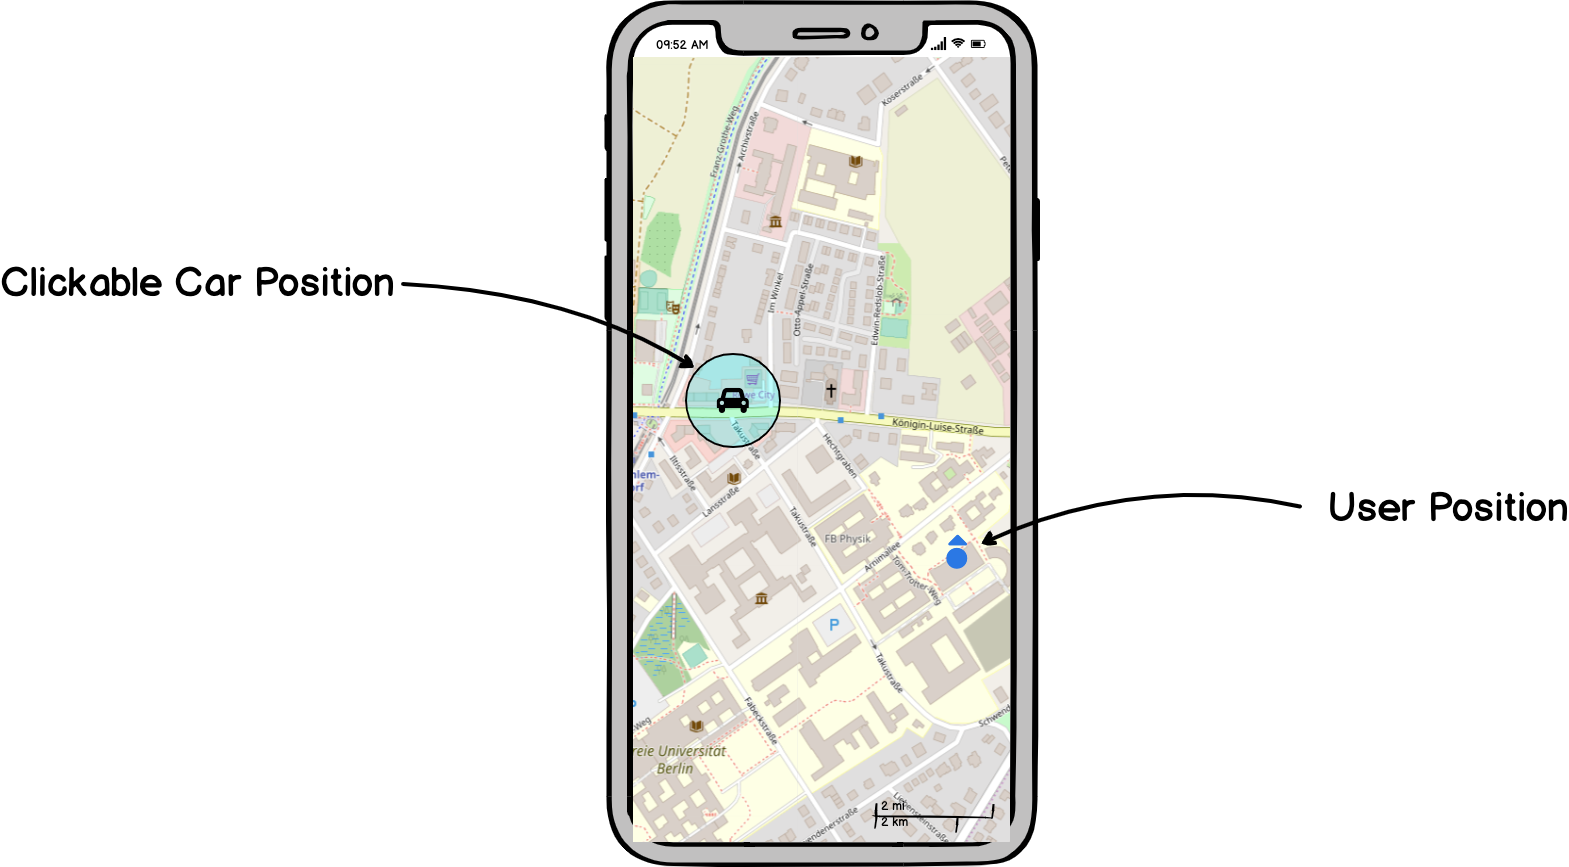
\includegraphics[width=0.75\textwidth]{images/UI/[I1V3]MapView-ParkingPositonDetermined.png}
    \caption{[I1V3] MapView - Parking Position Determined}
    \label{fig:i1v3}
\end{figure}


\begin{figure}[H]
    \centering
    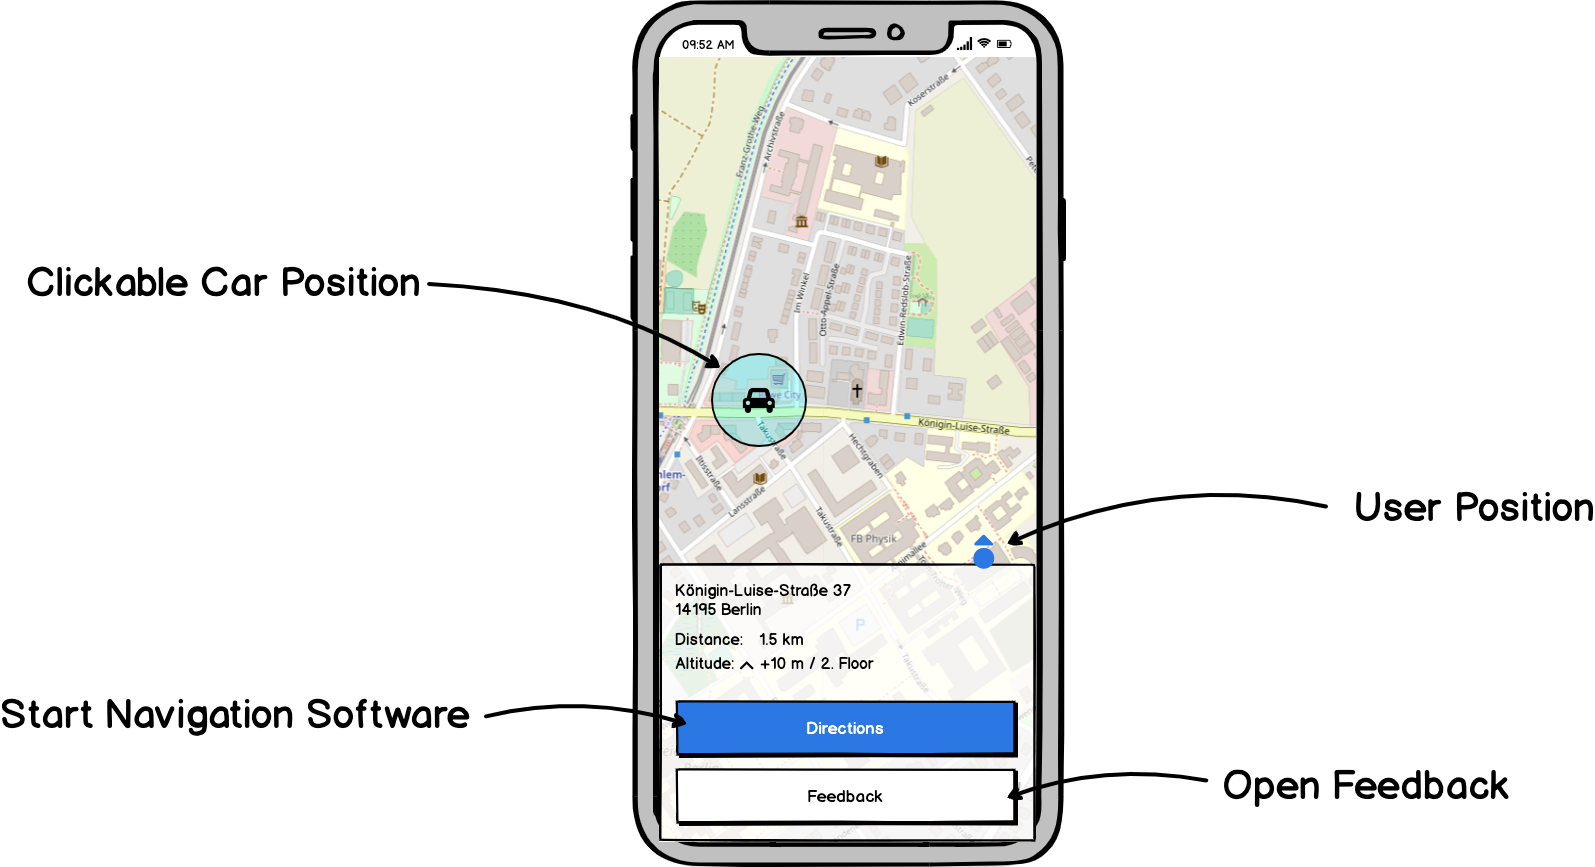
\includegraphics[width=0.75\textwidth]{images/UI/[I1V4]MapView-Details.png}
    \caption{[I1V4] MapView - Details}
    \label{fig:i1v4}
\end{figure}


The first iteration consist of five views. The storyboard of the user interface can be seen in Figure \ref{fig:i1story}. The application starts with the ''MapView - Loading'' view (cp. Figure \ref{fig:i1v1}). The view shows a map on which the location of the users marked. At the top of the page a string indicates the current loading state of the system. The string is included to make the state of the system visible. The map and the user location are shown to map the system to the real world. \cite{heurisitcNielsen}

If the application fails to determine the parking position, a pop-up menu is shown (cp. Figure \ref{fig:i1v2}) which notifies the user about the problem and explains the cause of the failure. 

On successful determination of the parking position, the view [I1V3] (cp. Figure \ref{fig:i1v3} is shown. View [I1V3] shows a map with the users location and the determined location of the users car. The label of the users car is clickable and opens [I1V4] (cp. Figure \ref{fig:i1v4}. 

[I1V4] presents more details about the determined parking position. It presents the address where the car is parked, the distance to the users car, the altitude difference between the user and the users car and the floor of the parked car. Two buttons are presented: One button opens a third party navigation software to navigate to the determined location, and a Feedback button, to report the accuracy of the determined parking position of the car. When the Feedback button is clicked, the application switches to view [I1V5] (cp. Figure \ref{fig:i1v5}).

\begin{figure}[H]
    \centering
    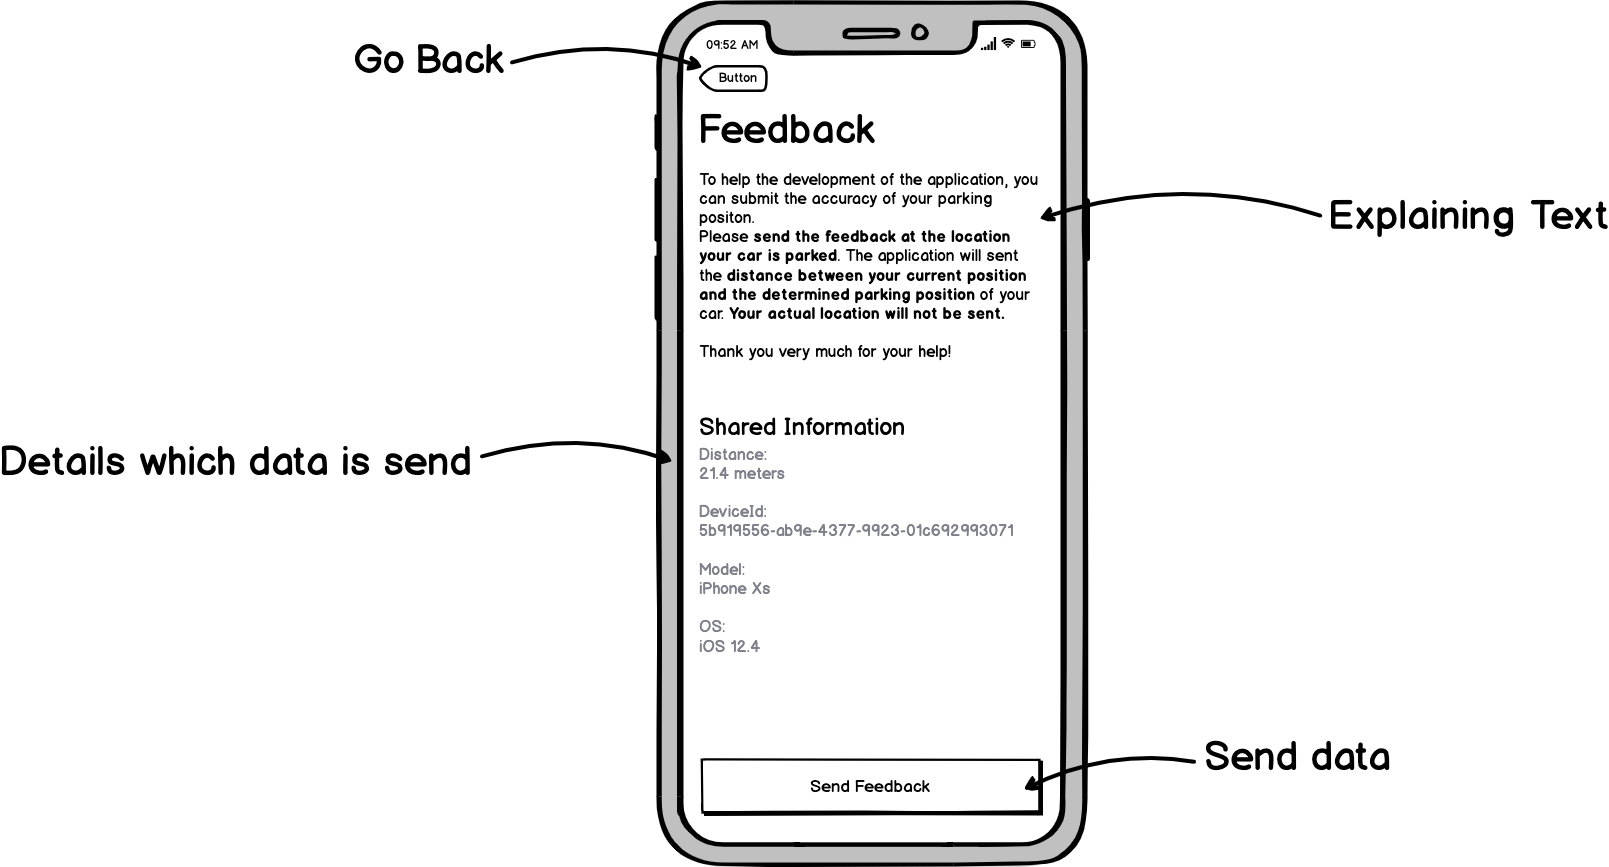
\includegraphics[width=0.75\textwidth]{images/UI/[I1V5]Feedback.png}
    \caption{[I1V5] Feedback}
    \label{fig:i1v5}
\end{figure}

[I1V5] presents the user instructions to report the accuracy of the determined parking position, the transmitted information and a button to report the information. When the button is clicked, the information is send and the application returns to view [I1V4]. The user can also go back to the previous screen without sending any information by using the Back button.


The think aloud protocol shows two problems of the user interface. First, in the view [I1V3], the user does not understand that the car icon is clickable. Second, the user expects to be able to give feedback in text form in view [I1V5].

\subsection{Iteration 2}

\begin{figure}[H]
    \centering
    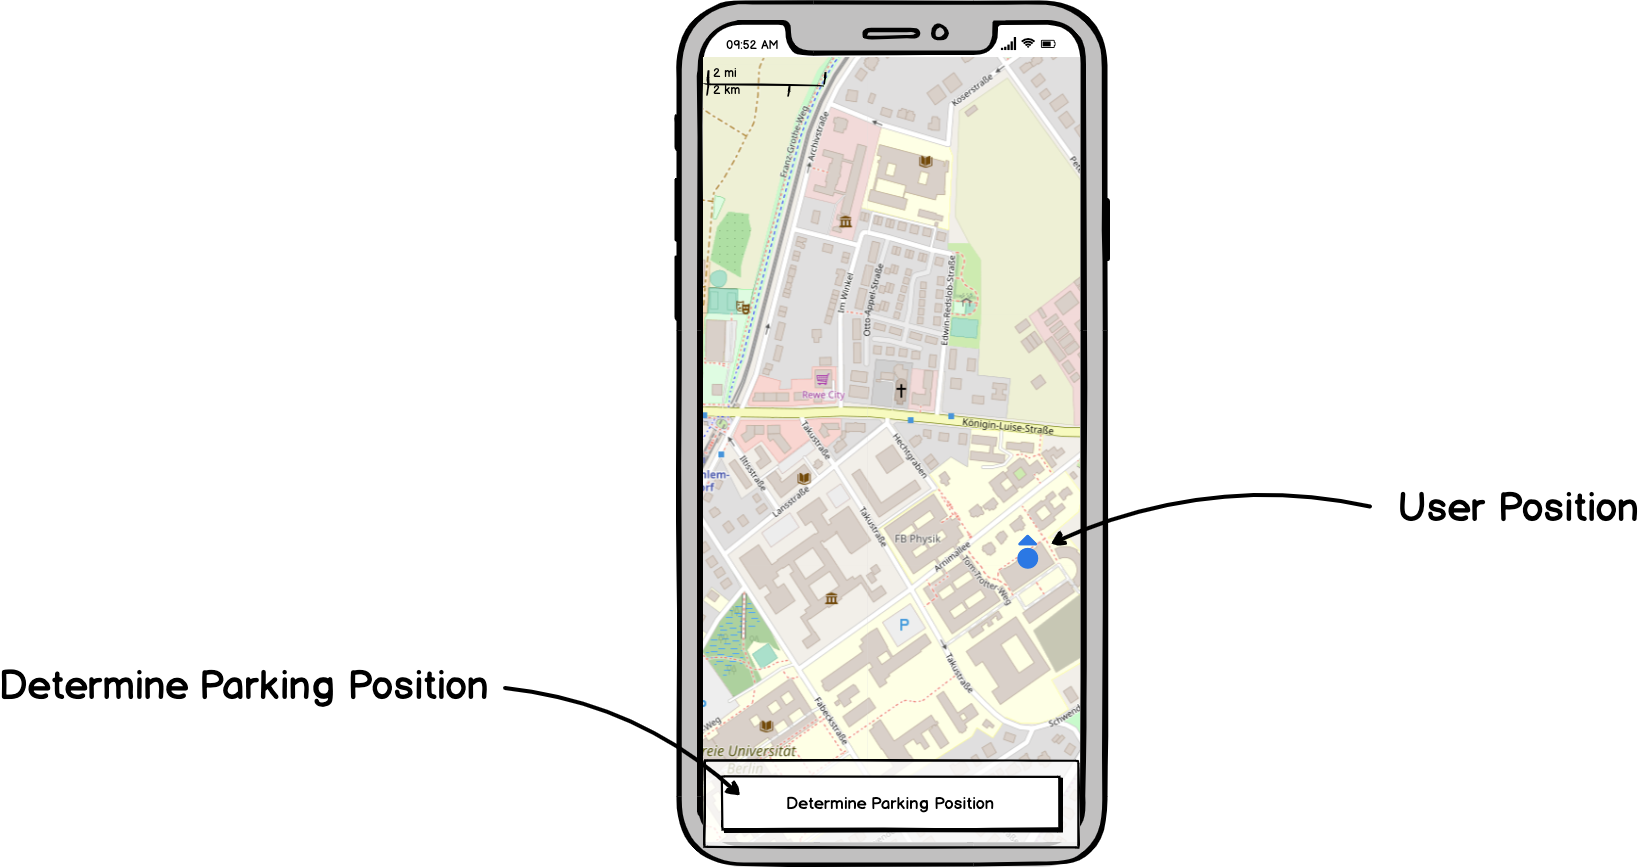
\includegraphics[width=0.75\textwidth]{images/UI/[I2V1]MapView-Loading.png}
    \caption{[I2V1] MapView - Loading}
    \label{fig:i2v1}
\end{figure}

\begin{figure}[H]
    \centering
    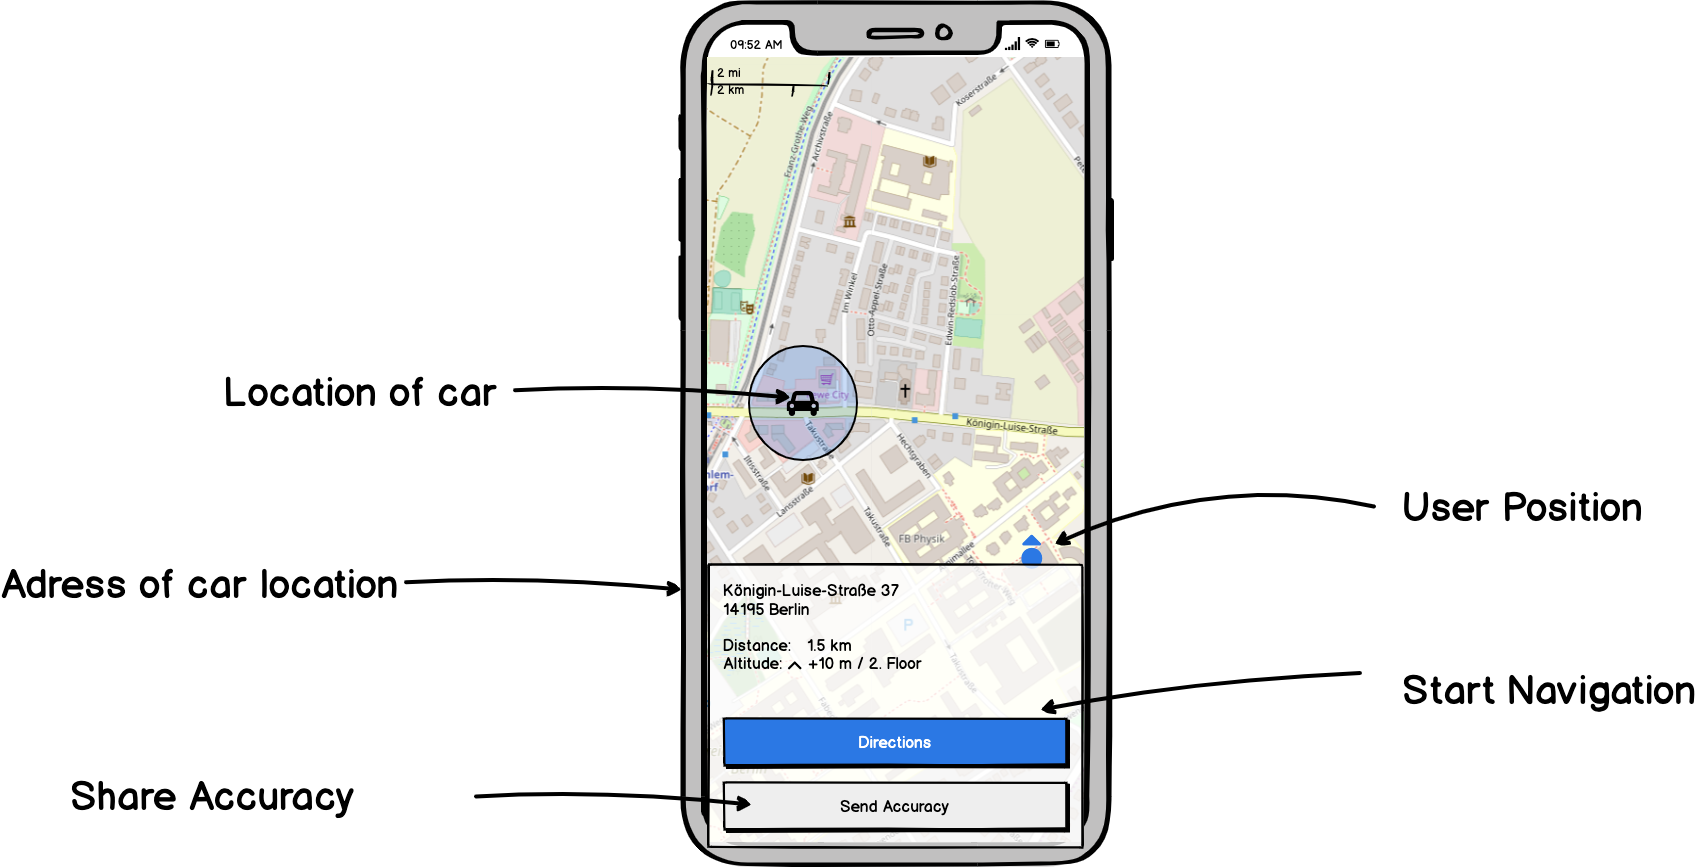
\includegraphics[width=0.75\textwidth]{images/UI/[I2V3]MapView-DeterminedParkingPosition.png}
    \caption{[I2V3] MapView - Determined Parking Position}
    \label{fig:i2v1}
\end{figure}



In the second iteration of the user interface, the two problems of Iteration 1 are improved. The view [I1V3] is removed completely in the second iteration. When the application determines the position of the car, the user interface presents directly the detailed information.  In view [I1V4], the call to action to send Feedback is rephrased to say  ''Send Accuracy'' to better represent the actual functionality. The headline of view [I1V5] is also changed to ''Send Accuracy''. Because most views with a map show a white partly transparent box on the bottom, the loading view is adapted to also show the box (cp. Figure \ref{fig:i2v1}). This is done to keep the interface consistency in the application. 

The think aloud protocol of the second iteration shows three obstacles. First, the altitude in [I2V3] is understood as total altitude of the car, but it shows the relative altitude of the car compared to the current altitude of the user. Second, the user is unsure if the = presented address in [I2V3] is the address of the location of the car but assumes so. Third, the user does not notice in [I2V4] that the accuracy is supposed to be reported at the actual parking position of the car.

\subsection{Iteration 3}


The third iteration improves on the three obstacles of the previous iteration. 
First, the altitude is separated into the two rows ''Relative altitiude'', which shows the relative altitude between the determined location of the parked car and the user location, and ''Floor'', which shows the floor in which the car is parked. Second, the headline ''Your car is parked at: '' is added to the details of the determined parking location to clarify that the shown information are information about the determined parking location. 

The think aloud protocol of the third iteration only shows one confusion: The call to action of the ''Send Accuracy'' is unclear

\subsection{Iteration 4}

To improve on the unclear call to action of the ''Send Accuracy'' button, the call to action is changed to ''Report Accuracy''.
